%\RequirePackage[l2tabu, orthodox]{nag}  %Checks for older packages 

\documentclass[11pt,a4paper]{article}
% \documentclass[10pt]{extreport} $ allos to make the font smaller
\usepackage[utf8]{inputenc}

\usepackage{amsmath}
\usepackage{amsfonts}
\usepackage{indentfirst}
\usepackage{amssymb}
\usepackage[font={footnotesize}]{caption} %Makes the captions small


%% Figures packages
\usepackage[pdftex]{graphicx}
\usepackage{float}   %Es para colocar el objeto flotante exactamente donde se ponga el comando con H
\usepackage{caption}
\usepackage{subcaption}
\graphicspath{{../results/}}
\usepackage{sidecap}  %Para poner figuras a los lados


\usepackage{setspace} % Needed for Pyton syntax highlight
\usepackage{listings}    % Include the listings-package, nice verbatim for code
\usepackage{color}
\usepackage{courier}


\usepackage{cleveref} %puts figure and equation appropiately \cref{} 

\usepackage{natbib} %For bibliography
%\usepackage{cite}
\usepackage{framed} % To use boxes, or frames around text

\usepackage{parskip} %Para saltos entre parrafos
\setlength{\parindent}{0pt} 
\setlength{\parskip}{\baselineskip}
\usepackage[a4paper,margin=0.8in]{geometry}  %%Cambiar los margenes

\newcommand{\HRule}{\rule{\linewidth}{0.5mm}}

%\usepackage{hyperref} %This should be loade after most of the other packages 
% \hypersetup{colorlinks=true}  %Para que los hiperlinks cuando se hagan referencias aparezcan en colores.

\definecolor{dkgreen}{rgb}{0,0.6,0}

\title{Lab12: DD2380 }
\author{
Ramon Heberto Martinez Mayorquin  hramon@kth.se 
}



\begin{document}

\begin{titlepage}
\begin{center}
%\includegraphics[width=0.15\textwidth]{logo}\\[1cm]    

\textsc{\LARGE Kungliga Tekniska högskolan}\\[1.0cm]

\textsc{\Large Computational Python 2015}\\[2.0cm]



\begin{figure}[H]
	\centering
 
\includegraphics[width=0.35\textwidth]{sese.png}
\end{figure}
%\\[1cm]    
%

% Title
\HRule \\[0.4cm]
{ \huge  Parameter Exploration for in-house library.
}\\[0.4cm]
\HRule \\[1.5cm]

% Author and supervisor

Author: Ram\'on  Mart\'inez  \\ 
\large Course Responsible: Olav Vahtras  \\ [2.5cm]
%\normalsize Presenta \\
%\large Supervisors 2: Jan Antolik \\[2.5cm]

\textsc{\Large School of Computer Science and Communication \\
PDC Center for High Performance Computing}\\ [1.0cm] 
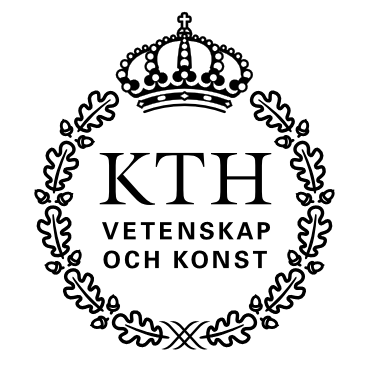
\includegraphics[width=0.15\textwidth]{KTH_black.png}\\[1.5cm] % Controls the distance till the new object 
% Bottom of the page
{\large 17th November of 2015}

\end{center}
\end{titlepage}



\begin{abstract}
This report is used to describe our work regarding tools for parameter
exploration in an in-house library. First we describe the data
processing pipeline that we use in this research. This describes the rather complicated process to make it more manageable and furthermore introduces the context. Once we do we can present the pairs of input and output that we want to store and describe the problem around this process. After that we present a brief discussion of the tools that we learn in the course and applied ot the problem here. To conclude we provide more technical details on how the how process is carried out and discuss the limitations of our framework.
\end{abstract}


\section{Problem.}\label{problem.}

\subsection{Spatio-temporal Structure}\label{spatio-temporal-structure}

We have a in-house library that functions mainly as a big pipeline for
data processing and exploration. The input of the data pipeline is composed of $N_{time\:series}$ time series each one with a sampling rate attached to it. To each of those time series we attach what we call a \textbf{lag structure}. The lag structure is a vector that
represents \textbf{how we believe the past of the signal affects the
present}. In more detail, the vector contains a series of lags that we
use to calculate the auto-correlation between the time series and the
time series shifted by quantities given on this vector. For example if the vector of lags is
the following lags = (1, 2, 3, ... ) then we can obtain the usual
auto-correlation function because all this shifts are given by the unit. In general we use the same lag vector for every signal and we will denote the dimension of that vector here as
($N_{lags}$) for further explanations.

In our use case the signals come from different points in space, so we can say that they
encode the spatial information. By adding a lag vector to each signal we
intend to also include some degree of temporal information. Our aim at the end is to
quantify how the different time series are related between
themselves in space and time. In order to do so we calculate a
cross-correlation matrix in the following way. For each possible lag and every possible
signal combination we calculate the cross-correlation between them. This
way we obtain a matrix with ($N_{time series} \times (N_{lags}$)
rows and the same amount of columns. We call this matrix the Spatio
Temporal Distance Matrix (\textbf{STDM}) and it provides a concrete
measure of the spatio-temporal relationships. Note that the for the same data we obtain a different temporal matrix depending on the lag structure that we chose.

Finally we would like to interpret our spatio-temporal relationships as
a \textbf{distance matrix}, in other words, we want our matrix to provide an idea of how close two time signals are. In the example above an given entry is going to be
big if the elements that represent the row and the column are highly
correlated. This is exactly the opposite of what we want. We want our
\textbf{elements to be far away if they are uncorrelated and to cluster
together if they are correlated}. So in order to interpret them as
distances we create another matrix where each entry is one minus the
absolute value of the old matrix. In other words $d_{ij} = 1 - | m_{ij}|$. This way we can directly interpret
this matrix as a distance measure between the spatial and temporal parts
as we initially intended.

\subsection{Embedding}\label{embedding}

At this stage of our analysis we have a distance matrix that represents
how all the sensors and the shifted in time versions of those sensors
are related. The next step in our pipeline is to apply the Multidimensional
Scaling Algorithm (\textbf{MDS}) in order to embed all the $N_{time\:
series} \times N_{lags}$ points in an euclidean space of dimension
$N_{embed}$. As a result of this process we just added an extra parameter $N_{embed}$ to our pipeline. 

\subsection{Spatio-Temporal Clustering.} \label{spatial-temporal-clustering.}

Now with all our points into an euclidean space we can partition the space of our sensor by a process of vector quantization. We do this in order to identify which groups of sensors cluster together. This is meaningful because if sensors cluster it is because they are highly correlated between themselves. In other words that group of sensors is statistically providing similar information. 

When doing this we have to
determine the number of partitions or cluster that our algorithm is going to produce. In other words we have introduced yet another parameter (or decision). We denote this number by  $N_{spatial\: clusters}$. After this process is
done we have each of the sensors and their respective lags associated
with a particular clusters. What we have created here is a
division of the spatio-temporal information according to the data it
provides. Furthermore we also have a mapping between each of the sensors in our space and a cluster and vice-verse. We use a dictionary for both data structures. For reasons that will be clarified later those two objects also required to be stored. 

\subsection{Data clustering.}\label{data-clustering.}

The final point is to partition the data as well. For each of the
clusters above we select a number \(N_{data\:clusters}\) that quantifies
how many clusters the data in that space will have. So for a given group
of sensor we consider all the data on that particular group and apply a
cluster algorithm to it. This gives us a partition of the map, in this particular case we are interested on the centers of each of the partitions, therefore we store a dictionary where each key is the cluster and the value is a list with the partition centers on it.

\section{Parameters.}\label{parameters.}

The first things that stands out with the description of the context above is the sheer
complexity of the problem. There are many bifurcations in the pipeline
and in order to cope with this complexity we need to come up with a
systematic way of dealing with the parameters. In the following we
identify all the parameters involved in order to run a trial of our pipeline. All of those are candidates for storage.

\subparagraph{Input parameters.}\label{input-parameters.}

\begin{itemize}
\item
  \textbf{Data} (This is also the data that characterizes the signal)
\item
  \(N_{spatial\:clusters}\)
\item
  \(N_{embedding\: space}\)
\item
  \(N_{data\: clusters}\)
\item
  lag structure ($t_i$, window size, type of filter)
\item
  time, dt
\end{itemize}

Now we also identify what the run is going to produce. 

\subparagraph{Output data}\label{output-data-to-visualize.}

\begin{itemize}
\item
  Matrix with the signals lagged
\item
  STDM
\item
  A map from each of the sensors to the cluster that it belongs.
\item
  The embedding of all the sensors in the euclidean space.
\item
  The center of the clusters in the data space.
\item
  A map that assigns to each spatial clustering a list of data clusters.
\end{itemize}

\subsection{The main problem.}\label{the-main-problem.}

The main problem is here is to attach to our pipeline a mechanism to
understand the role of the parameters in the data processing mechanisms.
In order to do so we need a systematized way of consistently storing the
data with the relevant parameters attach to it. Our first attempt at it
is just to produce a plot for each of the relevant graphs above. In the
following section I describe how this can be done using
\texttt{matpltlotlib}, version control and the tools that we learn to
use in the course.

\section{Python used and python
learned.}\label{python-used-and-python-learned.}

\subsection{Git branches}\label{git-branches}

The first thing to describe regarding the tools we used from the course is
version control. I have been using version control before but I was
doing it in a monolithic or mono-branch way. This was of working has a well know problem, if a new feature was created that deviated far enough from the
original (and working / functioning) project it is really hard to backtrack
appropriately. By creating a different branch to work with
experimental setups the whole process gets isolated. This possess the advantage that if things go out
of control too much, reverting back to business as usual is as easy as
changing branch and deleting the failed experiment. So in brief I learned how to
use multiple branches at git in order to deal experimental feature
development.

\subsubsection{Matplotlib}\label{matplotlib}

In order to take full advantage of the configuration of matplotlib it is
necessary to use it in its class oriented mode. For the visualization
tools for example I had a recurrent problem. When I first started
using the pipeline I created a function to display a visualization of every one of the
quantities above and only one of them. That is, each of the quantities had a segregated plot that used an entire figure for itself. However, when I wanted to do the
parameter exploration I realized that it would be very handy to combine
these plots into multigrid substructure (by this I mean the grid that
you get when you do something like subplot). This entailed a dilemma. Doing
that in the most straightforward way would imply building new functions
(one for each pair of relevant plots that I wanted to combine) in order
to display these two figures at the same time. This however went
directly against the principle of do not repeat yourself because the code would be for all purposes the same. Furthermore
what if in the future of the project I wanted to combine three instead of two figures
in one plot. if that was the case I will have to build yet another
function for each of the triplets and you can see from the combinatorial
explosion that that route was unlikely to scale well.

The way around this problem was to study the matplotlib object
model in detail. We realize then that in matplotlib we can decouple
the canvas from the contents of the visualization that we put in the canvas, in
matplotlib parlance we can just construct an axis like plot or an image
and then position them wherever we want into any canvas later with an
appropriate function. In short instead of coding again a function for
each of the plots we only make our normal functions to accept an axis as
an argument and if not figure is available we attach all the usual
content to the axis and return it. After returning we can position the
axis freely on the canvas with Gridspec for example or any other
convenience function that is fit for the job. With we have accomplished two things. First we have decoupled the figure creation from the actual state of the program. We can create arbitrary axis and pass them to the function so they attach the complete visualization to the axis. Second, if the axis is not present we can call the function in the usual way (axis=None) and they will create a figure and display it instantly.

\subsection{Decoupling of data products and datavisualization}\label{decoupling-of-data-products-and-data-visualization}

Yet another problem with our pipeline is the amount of memory and
computing time that it takes in order to go through even a simple
example. This means that doing the usual process of generating all the
data and gathering the complete output for all the possible parameters
was out of the table. The solution to that is \textbf{to decouple the
data generation process from the data visualization}. In this case we
first create the plots for a given combination of parameters and store
them. As the name of the file we use a string that involves a
combination of all the parameter used to create the signal. We save all
of those images in a folder with a time-stamp as title in order to make
the run unique and for retrieval purposes.

Now that we have all the set of images with a string characterizing
their parameters as a tittle we can access them systematically. The
classical way of doing this will be construct a GUI that just controls
the parameters and extracts the image with the unique string. It is well known that despite Python simplicity programming \textbf{graphical user interfaces} (GUI) still involves a lot of effort, boiler plate and usually increase the complexity of your  dependencies, all of this together requires developing time that is usually not available in a scientific programming environment.  

Fortunately Python provides an even faster way of doing the same tasks that fits most of the scientific use cases at hand. We can use the \textbf{Ipython.widgets} module in order to create sliders for some parameters of interest or a combination of them. In short using the ipython
notebook we have created and interactive environment that retrieves the
image that we need and displays it automatically allowing a smooth
exploration of parameters without the hassle of building a GUI to achieve the same end result.

\section{Final Discussion.}\label{final-discussion.}

We have describe here the process of building a parameter exploration
library. The tools that have helped us accomplishing this goal are the
class oriented capabilities of the matplotlib library and the
interactivity added to ipython notebook with the widgets package. With
those two and decoupling the data generation from the visualization part of our
pipeline we have facilitated the construction of complex routines. Furthermore we can run and study our results systematically later without memory constrains.

A problem with this approach is that the images that we store take quite
a bit space and are not reproducible. That is, the step from data to
image is irreversible. A further step ahead will be to store the data
instead of the images as the end results of our pipeline. In order to accomplish this we store most of the important data matrices generated in the process in the \textbf{HDF} format. In order to this we profit from the capabilities provided by the Python library \textbf{h5py}. With this scheme we have been able to store all the homogeneous data produces in our simulations and then recover it down the line for further analysis. With this we have achieved to store our data in a persistent and standardized format reducing drastically the hard drive footprint of our simulations. Furthermore the h5py library allow us to integrate all of this in our code in Python friendly way consistent with our previous framework.


\bibliographystyle{plainnat}
\bibliography{references}
\end{document}
